\documentclass[a4paper]{article}

\usepackage{graphicx}
\usepackage[utf8]{inputenc}
\usepackage[T1]{fontenc}
\usepackage[francais]{babel}
\usepackage[a4paper]{geometry}
\usepackage{float}
\usepackage{url}

\title{Editeur de niveaux Prog \& Play\\ Documentation Utilisateur}
\author{Benjamin BONTEMPS}

\sloppy

\begin{document}

\maketitle

\tableofcontents

\newpage

\section{Lancement de l'éditeur}
\paragraph{ }
Pour démarrer l'éditeur de niveaux de Prog \& Play, il faut tout d'abord s'assurer que tous les fichiers nécessaires à son bon fonctionnement sont présents :
\begin{itemize}
\item L'archive \textit{PPLE\_Launcher.sdz} doit être présente dans le répertoire \textit{<Spring>/mods/} (82.5.1) ou \textit{<Spring>/games/} (98+). Cette archive constitue le mod "Launcher", qui permet donc de lancer l'éditeur dans de bonnes conditions.
\item Pour les versions de Spring 98+, le dossier \textit{pp\_editor} doit être présent à la racine de Spring. Il contient des fichiers nécessaires au lancement de l'éditeur (dans \textit{editor\_files}), des fichiers nécessaires à la création de l'archive finale (dans \textit{game\_files}) et les niveaux et scénarios créés (respectivement dans \textit{missions} et \textit{scenarios}). Il est à noter que les dossiers \textit{editor\_files} et \textit{game\_files} ne sont pas nécessaires dans la version 82.5.1, et que les dossiers \textit{missions} et \textit{scenarios} seront créés automatiquement.
\item Au moins un mod pour Spring (\textit{Kernel Panic 4.1} par exemple) doit être présent dans le répertoire \textit{<Spring>/mods/} (82.5.1) ou \textit{<Spring>/games/} (98+). Celui-ci servira de base pour créer les niveaux.
\end{itemize}
\paragraph{ }
Une fois que ceci est fait, il suffit de lancer Spring, puis de lancer le mod \textit{Prog \& Play Level Editor Launcher 1.0} (voir Figure \ref{fig:editor-spring-launcher}). (Il vous sera demandé de choisir une carte et une IA. Ces dernières n'ayant aucune influence sur la suite, n'importe lesquelles feront l'affaire.)
\begin{figure}[H]
\centering
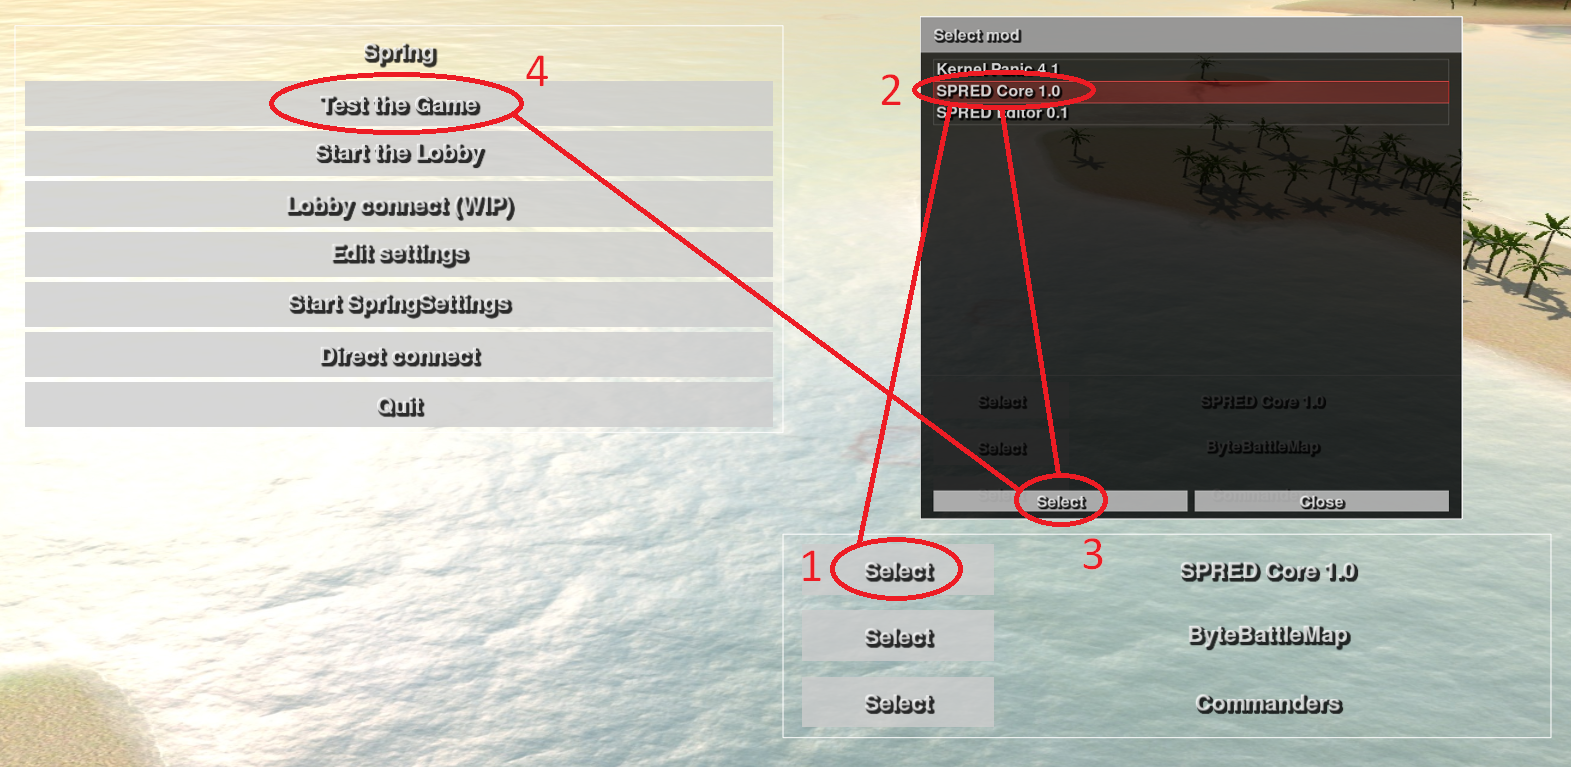
\includegraphics[width=\linewidth]{editor-spring-launcher.png}
\caption{Écran d'accueil de Spring.}
\label{fig:editor-spring-launcher}
\end{figure}
\paragraph{ }
Enfin, il vous sera demandé de sélectionner un mod parmi ceux présents dans le dossier \textit{<Spring>/mods/} (82.5.1) ou \textit{<Spring>/games/} (98+) (voir Figure \ref{fig:pre-launcher}). Ce mod sert à définir le jeu de base sur lequel seront créés les niveaux pour Prog \& Play (définition des unités et de leur comportement). Une fois ce mod sélectionné, Spring redémarrera sur l'éditeur à proprement parler.
\begin{figure}[H]
\centering
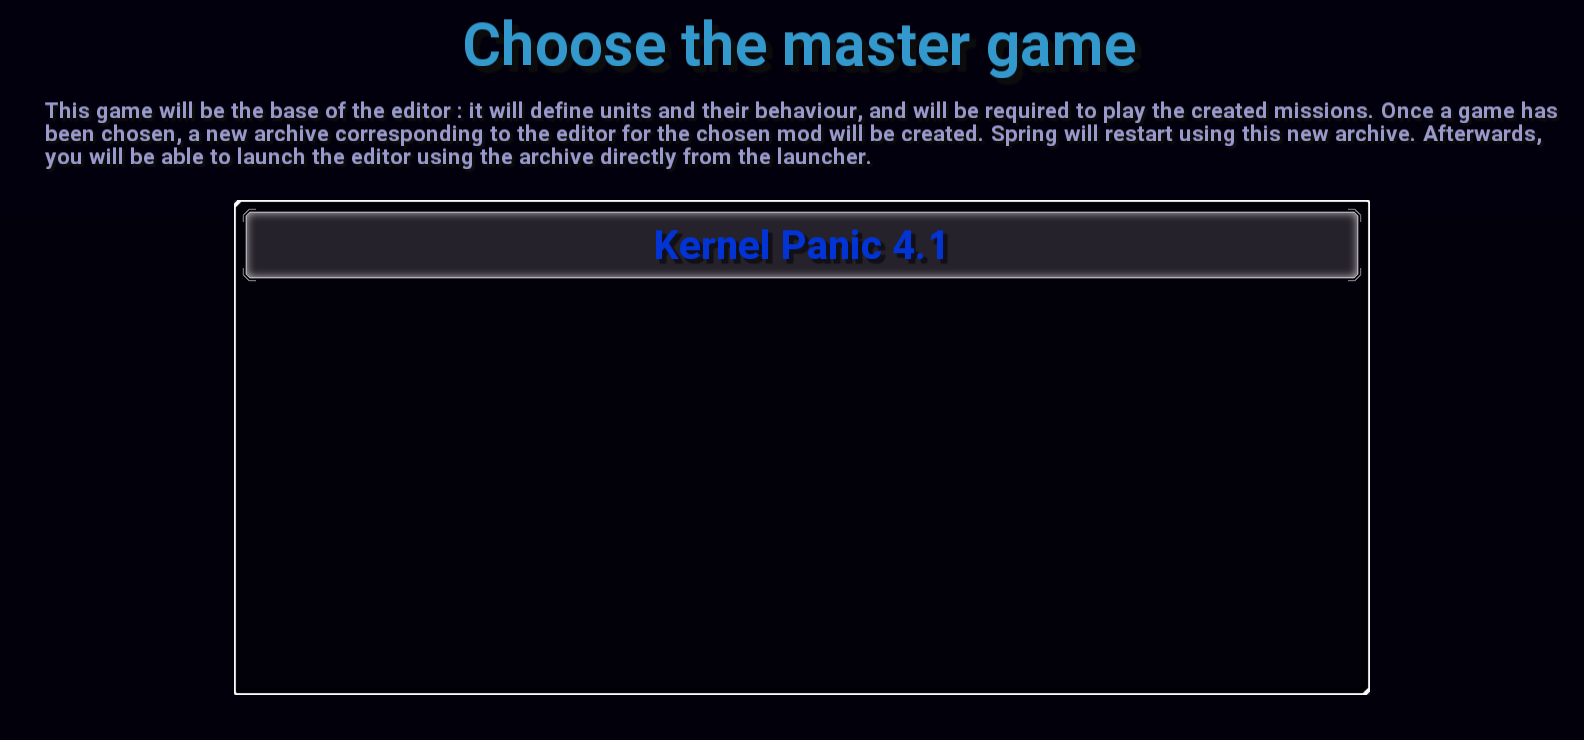
\includegraphics[width=\linewidth]{pre-launcher.png}
\caption{Choix du mod de base pour l'éditeur.}
\label{fig:pre-launcher}
\end{figure}
\section{Launcher propre au mod sélectionné}\label{launcher}
\paragraph{ }
Le launcher se divise en 3 menus distincts : Création d'un nouveau niveau, Modification d'un niveau existant et Éditeur de scénario (voir Figure \ref{fig:launcher-main}).
\begin{figure}[H]
\centering
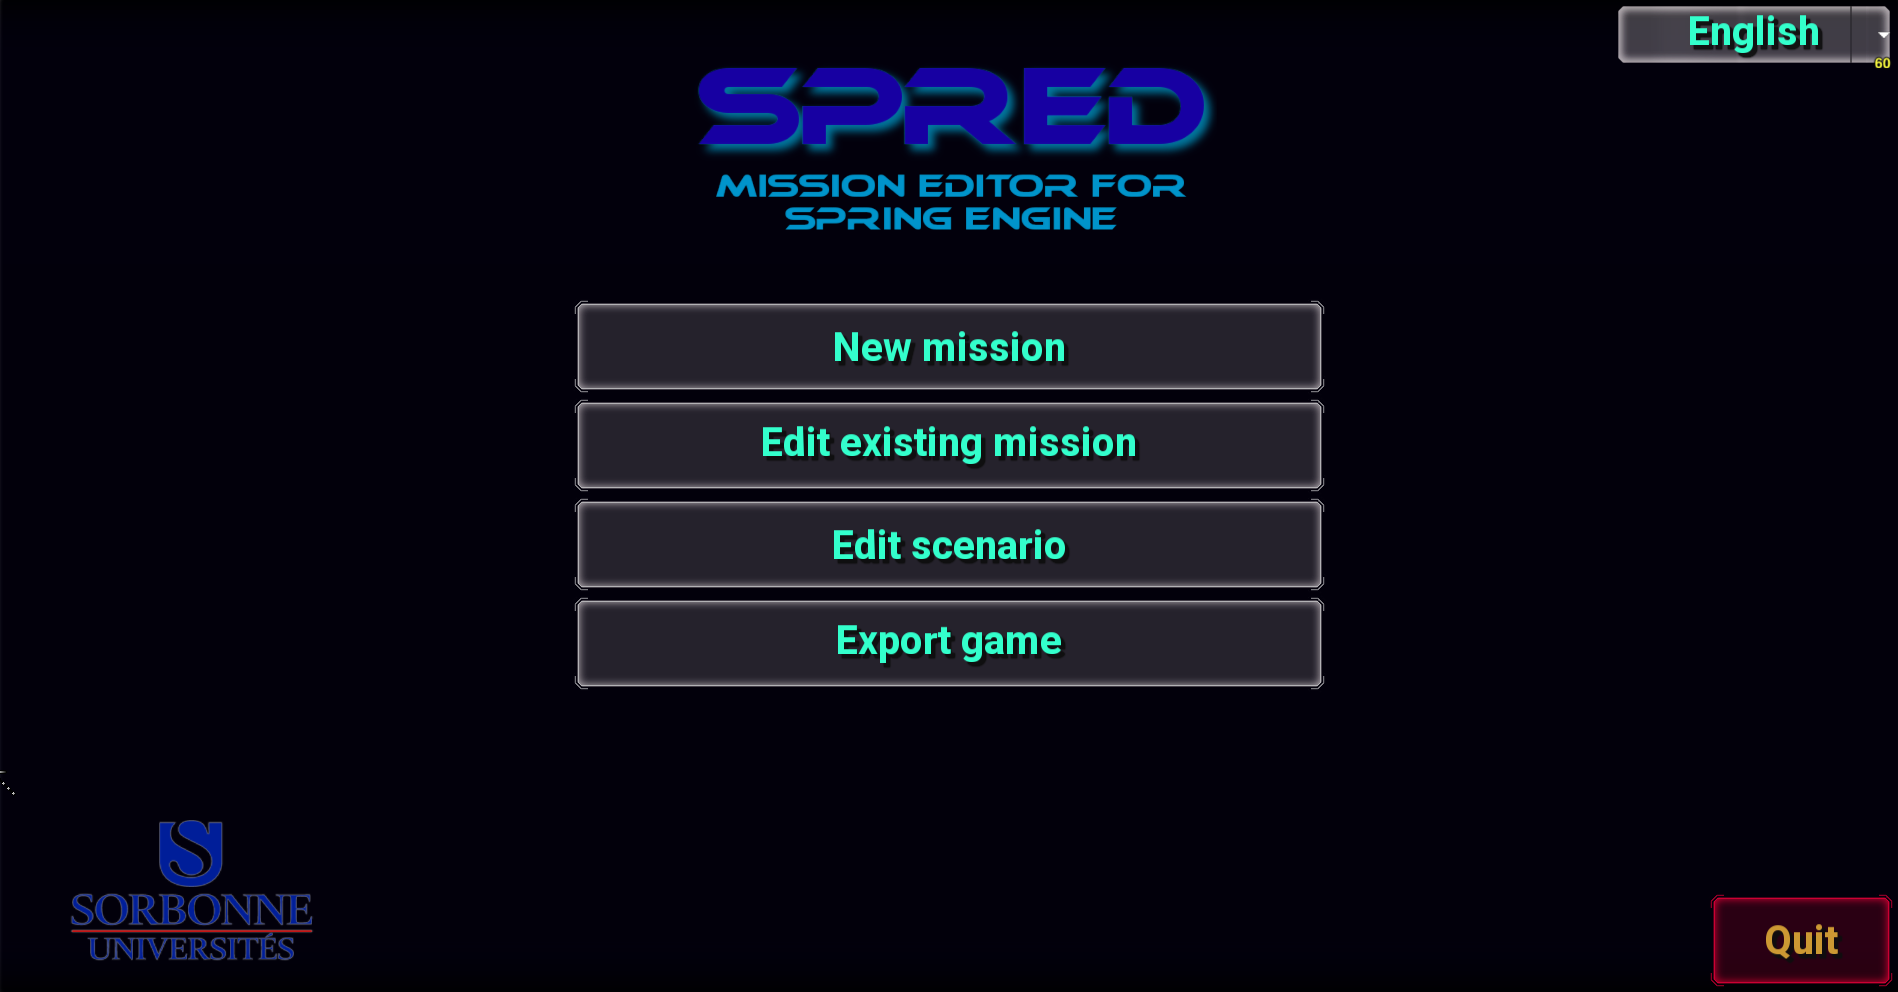
\includegraphics[width=\linewidth]{launcher-main.png}
\caption{Launcher de l'éditeur.}
\label{fig:launcher-main}
\end{figure}
\subsection{Création d'un nouveau niveau}
\paragraph{ }
Ce menu permet de choisir la carte sur laquelle vous voulez créer un nouveau niveau. L'ensemble des cartes disponibles correspond aux cartes présentes dans le répertoire \textit{<Spring>/maps}. Lorsque vous aurez sélectionné une carte, vous basculerez sur l'éditeur de niveaux, et vous pourrez commencer à créer votre mission (voir Section \ref{editor}).
\subsection{Modification d'un niveau existant}
\paragraph{ }
Ce menu permet de choisir une mission préalablement créée via l'éditeur. L'ensemble des missions proposées correspond aux missions présentes dans le répertoire \textit{<Spring>/pp\_editor/missions}. Les missions recensées sont celles ayant été créées pour le mod de base préalablement choisi.
\subsection{Éditeur de scénario}
\paragraph{ }
L'éditeur de scénario permet de scénariser les missions créées avec l'éditeur de niveaux. Vous trouverez plus d'informations concernant son fonctionnement à la section \ref{scenario-editor}.
\section{Éditeur de niveaux}\label{editor}
\paragraph{ }
L'éditeur se décompose en plusieurs menus distincts (voir Figure \ref{fig:editor-topbar}). Les parties suivantes s'attachent à décrire le fonctionnement et l'intérêt de chacun des menus.
\begin{figure}[H]
\centering

\includegraphics[width=\linewidth]{editor-topbar.png}
\caption{Barre de menus de l'éditeur.}
\label{fig:editor-topbar}
\end{figure}
\subsection{Fichier}
\paragraph{ }
Les fonctions de ce menu sont assez classiques :
\begin{itemize}
\item \textbf{Nouveau} - Permet de créer un nouveau niveau sur une carte sélectionnée parmi une liste déroulante.
\item \textbf{Ouvrir} - Permet de modifier un niveau ayant déjà été créé. Seuls les niveaux ayant été créés pour le mod de base sélectionné dans le launcher apparaitront dans la liste déroulante.
\item \textbf{Enregistrer} - Permet de sauvegarder le niveau dans le fichier \textit{<Spring>/pp\_editor/ missions/<Nom du niveau>.editor}.
\item \textbf{Menu principal} - Permet de retourner au launcher propre au mod sélectionné (voir Section \ref{launcher}).
\item \textbf{Quitter} - Permet de quitter l'éditeur et Spring.
\end{itemize}
\subsection{Unités}
\paragraph{ }
Ce menu permet d'ajouter, de déplacer et de supprimer des unités, ainsi que de modifier certains de leurs attributs (Figure \ref{fig:editor-units}). Il est également possible de les ajouter à des groupes d'unités pour une utilisation ultérieure dans les évènements (Figure \ref{fig:editor-groups}).
\begin{figure}[H]
\centering
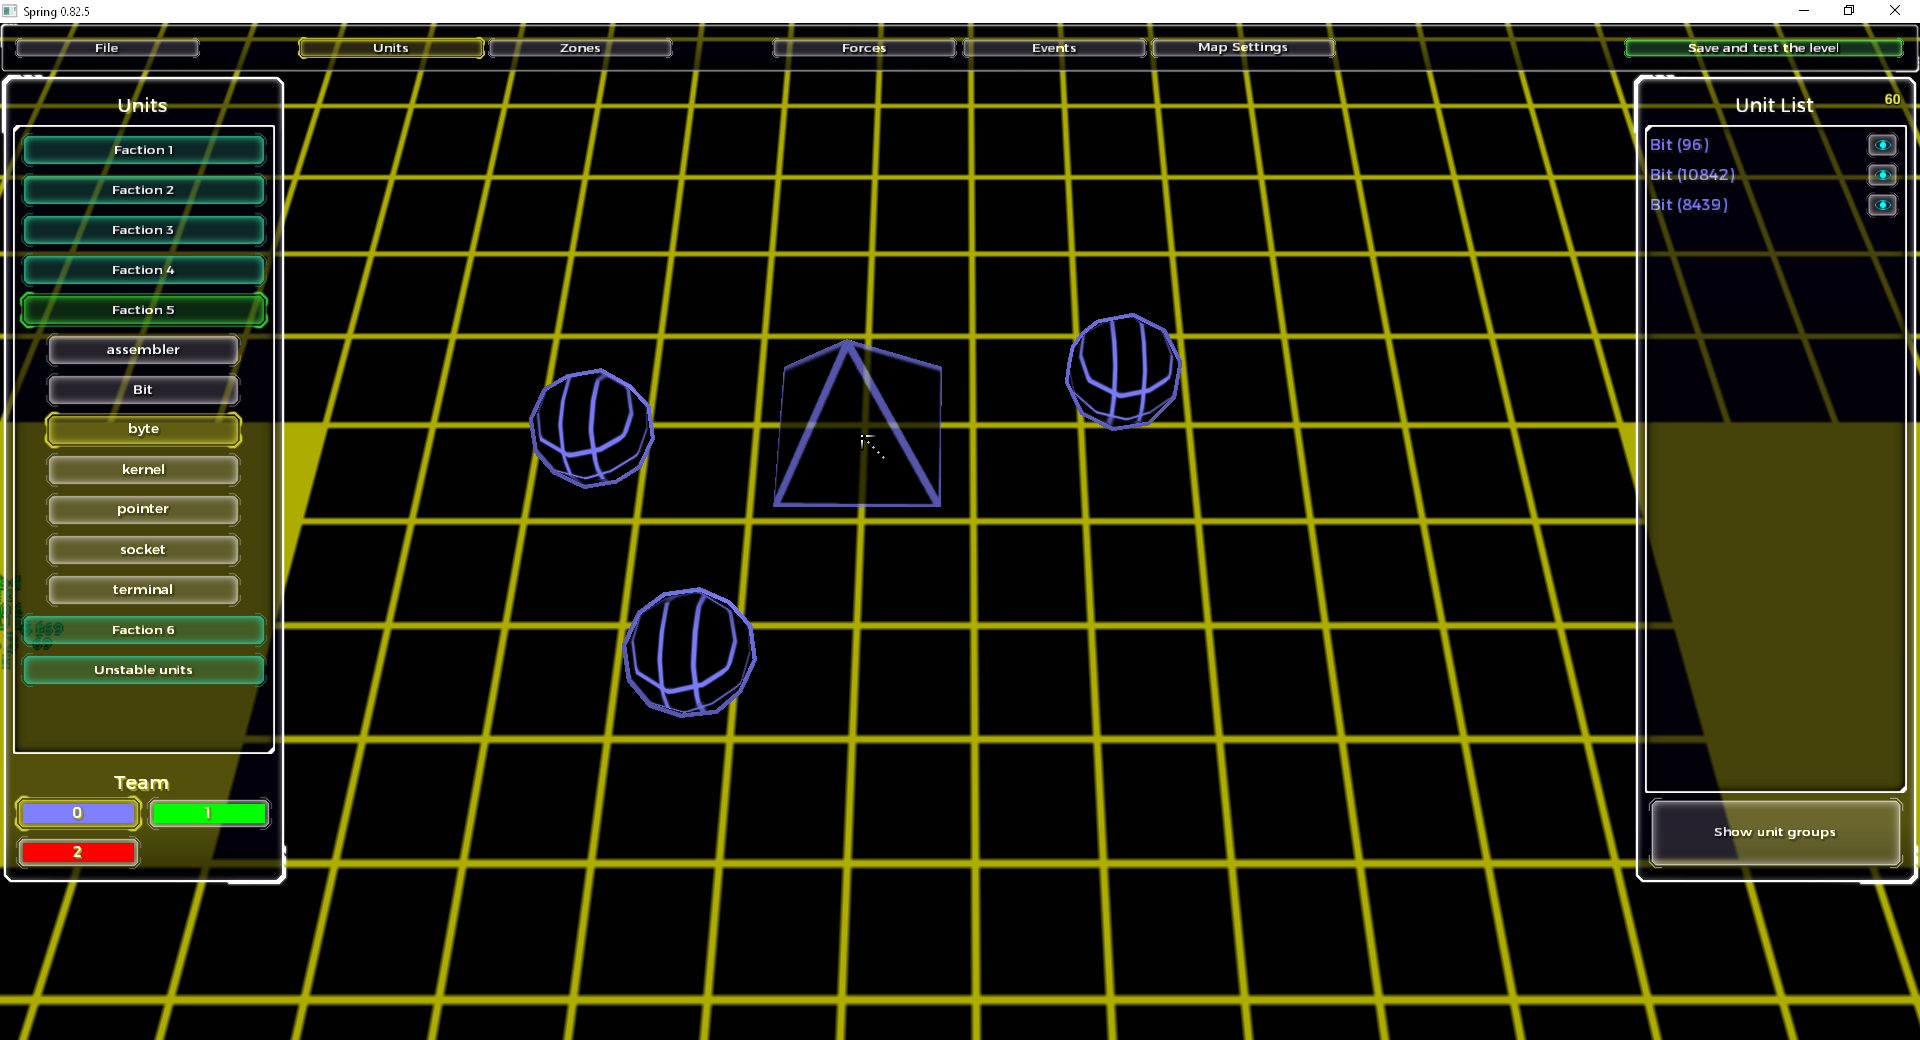
\includegraphics[width=\linewidth]{editor-units.png}
\caption{Interface de gestion des unités.}
\label{fig:editor-units}
\end{figure}
\paragraph{ }
Le menu de gauche permet de sélectionner un type d'unité et une équipe, et il est ensuite possible d'instancier une unité du type sélectionné qui appartient à l'équipe sélectionnée. Les types d'unité sont classés par faction. Une fois que des unités se trouvent sur le terrain, il est possible de les sélectionner\footnote{Il existe différents processus de sélection : il est possible de sélectionner une seule unité en cliquant dessus et plusieurs unités en cliquant sur chacune d'entre elles en laissant CTRL ou SHIFT enfoncé. Il est aussi possible de sélectionner plusieurs unités dans un rectangle en dessinant un rectangle de sélection par cliquer-glisser.} pour :
\begin{itemize}
\item les déplacer par cliquer-glisser ou en utilisant les flèches directionnelles.
\item les pivoter par cliquer-glisser en laissant enfoncer CTRL (pour toutes les faire regarder en direction de la souris) ou ALT (pour les faire regarder dans la même direction). Pour ces deux modes d'interaction, faites bien attention à partir de l'unité pour faire le cliquer-glisser. 
\item les supprimer en appuyant sur SUPPR.
\item modifier certains de leurs attributs (changement d'équipe, nombre de points de vie initiaux en pourcentage, activation ou désactivation des soins automatiques) en accédant au menu contextuel via un clic droit.
\item les ajouter ou les retirer d'un groupe d'unités.
\end{itemize}
\paragraph{ }
Les groupes d'unités peuvent être gérés plus précisément en utilisant l'interface accessible par le menu de droite. Pour ajouter des unités à des groupes, il faut sélectionner les groupes en question (1), sélectionner les unités que l'on veut ajouter (2), puis cliquer sur la flèche (3). Ces groupes sont purement logiques et servent à effectuer des actions ou à tester des conditions sur plusieurs unités en même temps.
\begin{figure}[H]
\centering
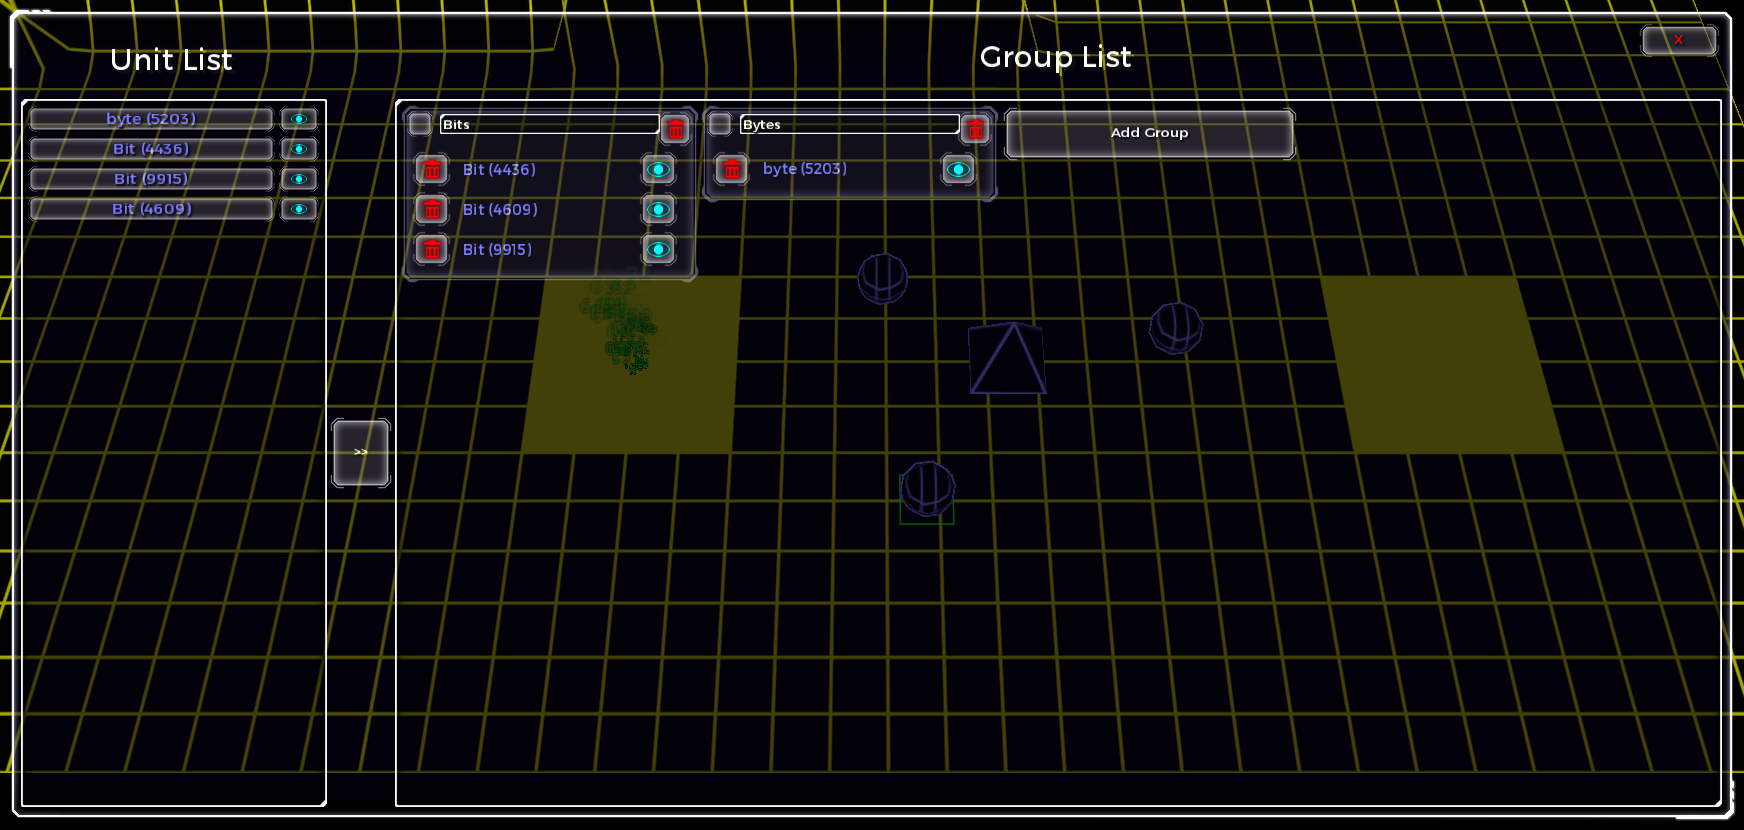
\includegraphics[width=\linewidth]{editor-groups.png}
\caption{Interface de gestion des groupes d'unités.}
\label{fig:editor-groups}
\end{figure}
\subsection{Zones}
\paragraph{ }
Ce menu permet de définir des zones logiques pour une utilisation ultérieure dans les évènements (Figure \ref{fig:editor-zones}).
\begin{figure}[H]
\centering
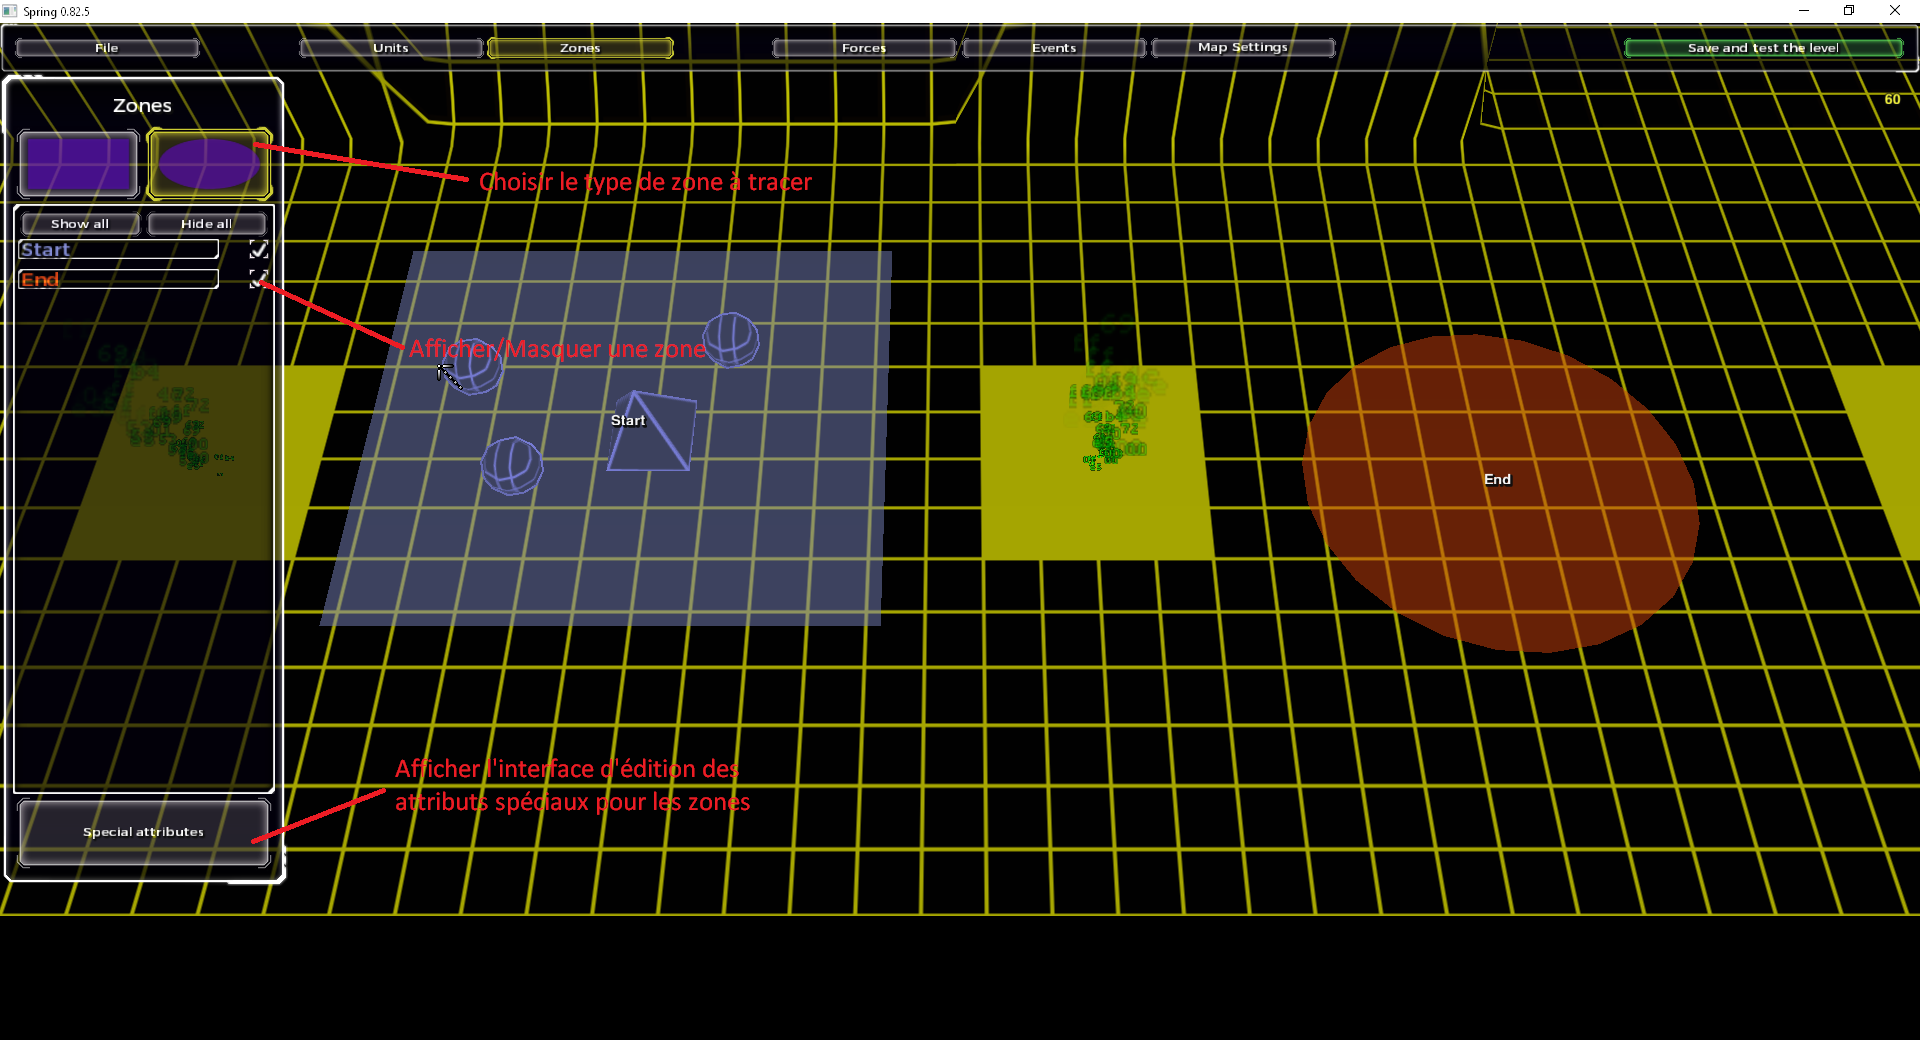
\includegraphics[width=\linewidth]{editor-zones.png}
\caption{Interface de gestion des zones logiques.}
\label{fig:editor-zones}
\end{figure}
\paragraph{ }
Les zones peuvent être rectangulaires ou elliptiques en fonction des besoins. De façon similaire aux unités, il est possible de les tracer (sélectionner le type de zone, rectangulaire ou elliptique, puis tracer la zone sur la carte par cliquer-glisser), de les déplacer, de les redimensionner (sélectionner une zone existante dans la scène puis utiliser les poignées de redimensionnement situées sur le pourtour de la zone pour modifier sa taille), de les renommer et de les supprimer. Chaque zone possède également des attributs spéciaux (Figure \ref{fig:editor-zones-special}) qui permettent d'afficher un marqueur portant le nom de la zone pendant l'exécution du jeu ou d'afficher en permanence le centre de la zone dans le champ de la caméra (dans le cas d'une caméra automatique, voir Section \ref{mapsettings}).
\begin{figure}[H]
\centering
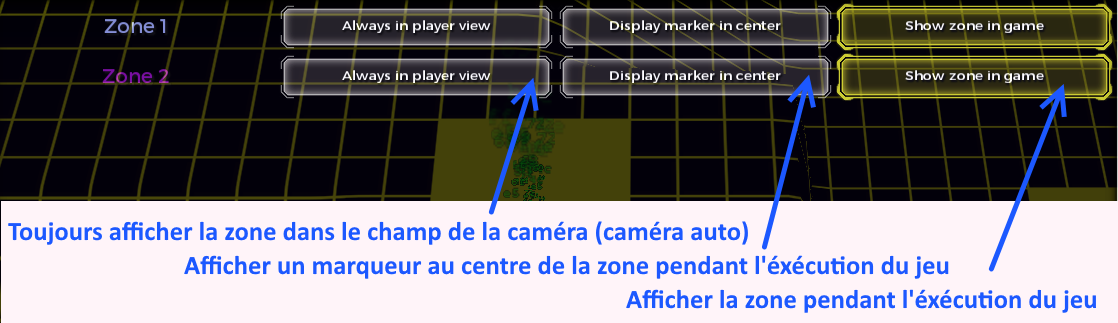
\includegraphics[width=\linewidth]{editor-zones-special.png}
\caption{Interface de gestion des attributs spéciaux des zones logiques.}
\label{fig:editor-zones-special}
\end{figure}
\subsection{Forces}
\paragraph{ }
Ce menu permet de gérer le statut des différentes équipes (Figure \ref{fig:editor-teamconfig}) et les alliances (Figure \ref{fig:editor-allyteam}).
\paragraph{ }
Chaque équipe peut être activée ou désactivée et contrôlée par un joueur ou par l'ordinateur selon les besoins. Il est également possible de changer le nom de l'équipe ainsi que sa couleur pendant l'exécution du jeu (la couleur dans l'éditeur restera la même). Dans le cas d'une équipe contrôlée par l'ordinateur, il est possible de spécifier le nom d'une intelligence artificielle pour la contrôler (optionnel)\footnote{Il s'agit d'une fonctionnalité très avancée.}. Pour que l'IA soit prise en compte dans le jeu, il faut :
\begin{itemize}
\item Soit simplement indiquer le nom d'une IA déjà incluse dans le mod de référence (vous pouvez regarder dans le fichier LuaAI.lua présent à la racine du mod de référence).
\item Soit créer sa propre IA (voir \url{https://springrts.com/wiki/AI:Development:Lang:Lua}) et intégrer cette nouvelle IA au jeu exporté.
\end{itemize}
\begin{figure}[H]
\centering
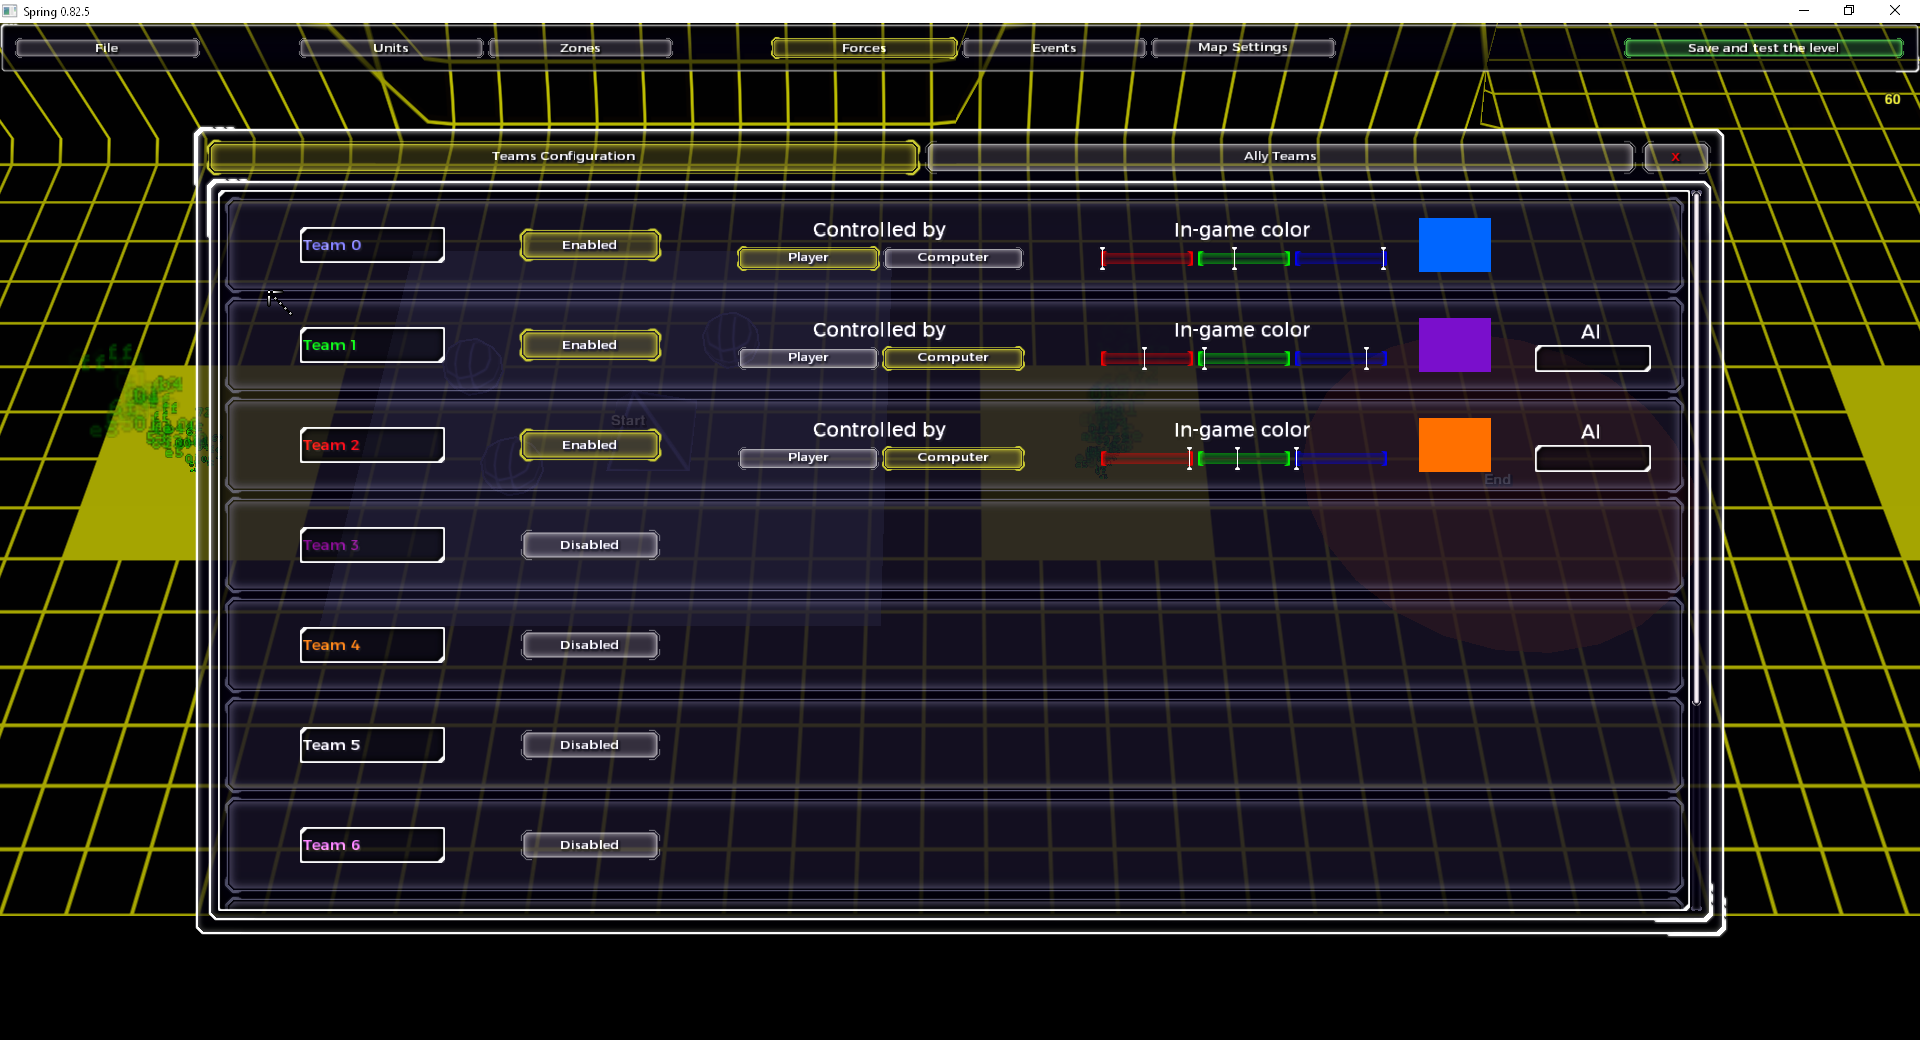
\includegraphics[width=\linewidth]{editor-teamconfig.png}
\caption{Interface de configuration des équipes.}
\label{fig:editor-teamconfig}
\end{figure}
\paragraph{ }
Les équipes peuvent être alliées entre elles. Il faut néanmoins noter que la notion d'alliance n'est pas réciproque : l'équipe 1 peut considérer l'équipe 2 comme son alliée tandis que l'équipe 2 considère l'équipe 1 comme ennemie. Initialement, les équipes ne sont pas alliées entre elles.
\begin{figure}[H]
\centering
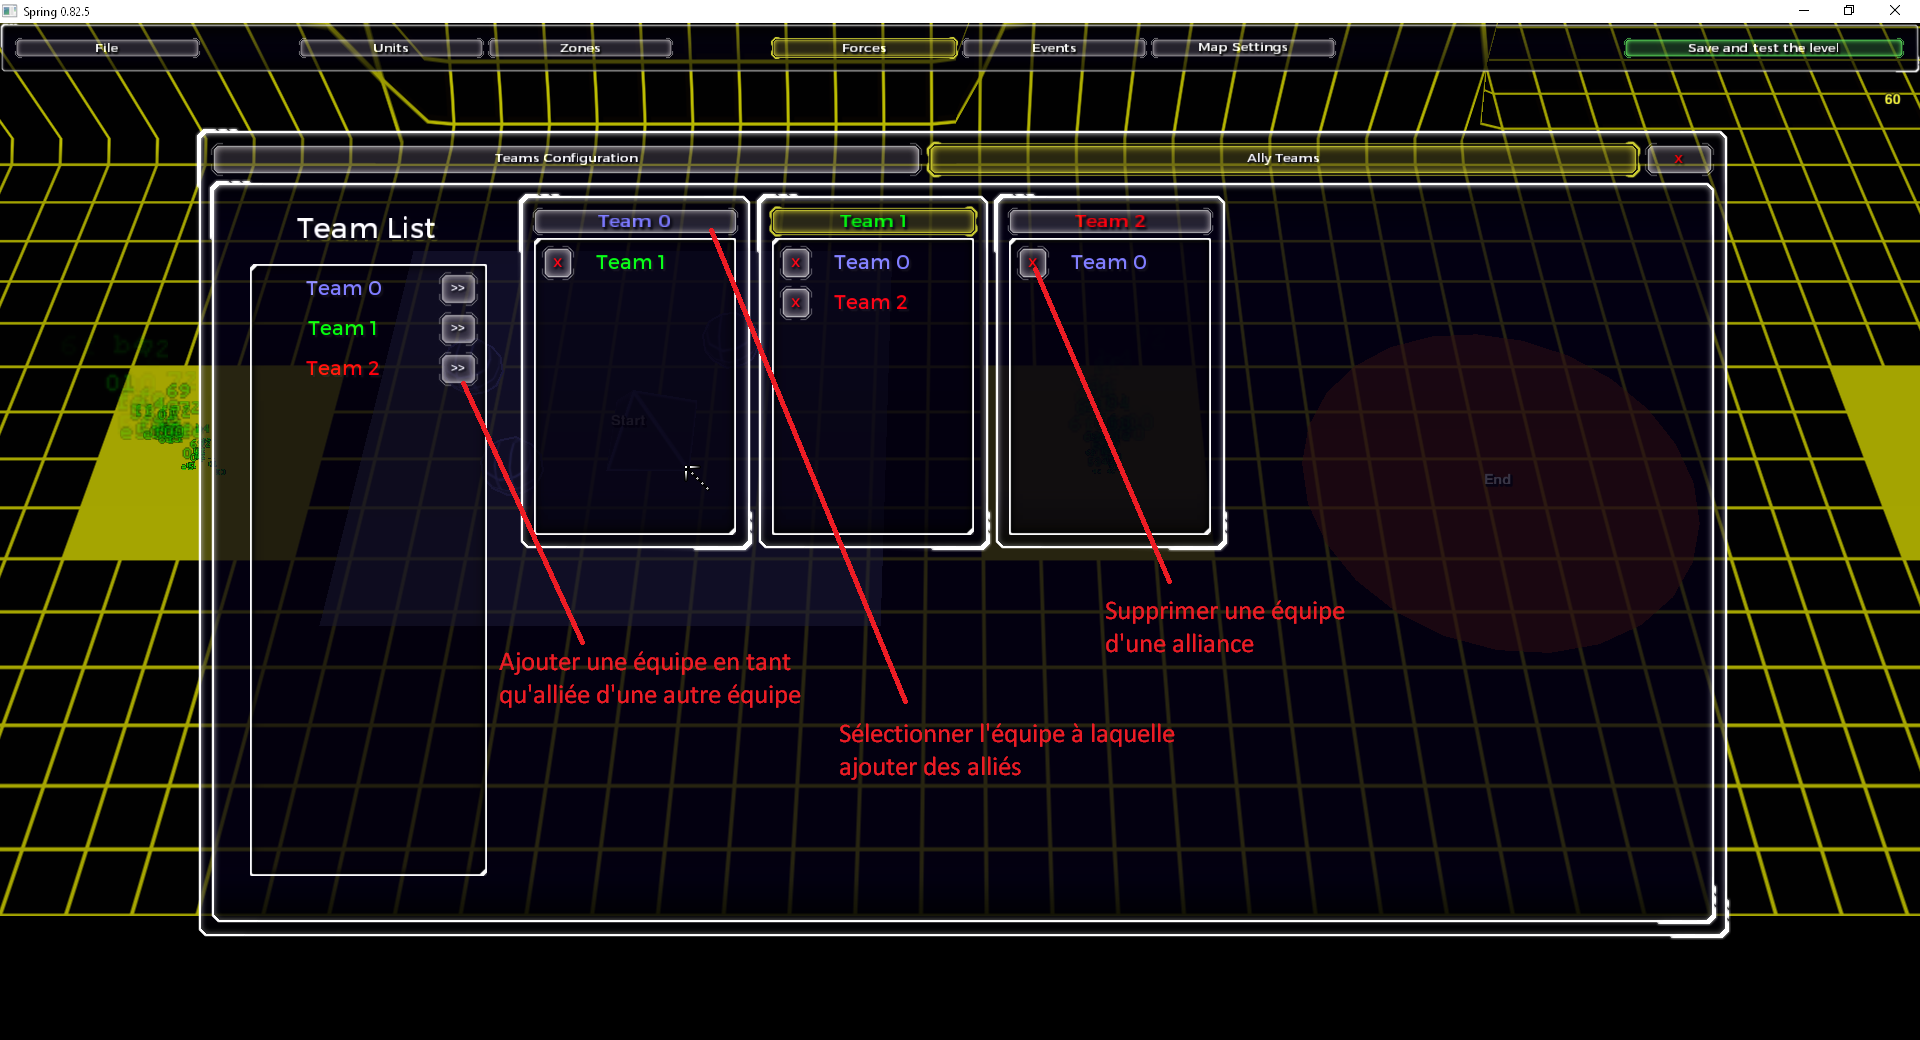
\includegraphics[width=\linewidth]{editor-allyteam.png}
\caption{Interface de gestion des alliances.}
\label{fig:editor-allyteam}
\end{figure}
\subsection{Évènements}
\paragraph{ }
Ce menu permet de gérer les différents évènements s'effectuant au cours de la mission.
\subsubsection{Évènements, conditions et actions}
\paragraph{ }
Un évènement correspond à un couple ensemble de conditions / ensemble d'actions. Il est possible d'ajouter des conditions et des actions puis de les paramétrer en utilisant les boutons et fenêtres appropriés. Un exemple est disponible Figure \ref{fig:editor-trigger}. Les actions et les conditions peuvent être plus facilement retrouvées dans la liste en choisissant un filtre correspondant au type de l'action ou de la condition (par exemple, si on veut définir une action portant sur des unités, on peut sélectionner le filtre "Unités" pour n'afficher que les actions portant sur des unités).
\paragraph{ }
Ensuite, il est possible de paramétrer l'évènement en définissant un déclencheur qui correspond à une expression logique entre toutes les conditions. Par défaut, le déclencheur est un ET logique global\footnote{Par exemple, pour un évènement possédant 3 conditions C1, C2 et C3, le déclencheur par défaut sera (C1 ET C2 ET C3).}. Lorsque le déclencheur renvoie \textit{"true"}, les actions s'effectuent l'une après l'autre, dans l'ordre où elles ont été définies. Cet ordre est paramétrable dans la même fenêtre que la définition du déclencheur (voir Figure \ref{fig:editor-eventconfig}).
\paragraph{ }
Il est également possible de changer les paramètres de répétition d'un évènement (une fois que l'événement s'est déclenché, si le paramètre de répétition est activé, l'événement pourra se redéclencher X secondes plus tard si le déclencheur est toujours valide), ainsi que d'ajouter un commentaire qui pourra servir lors de la modification ultérieure du niveau.
\begin{figure}[H]
\centering
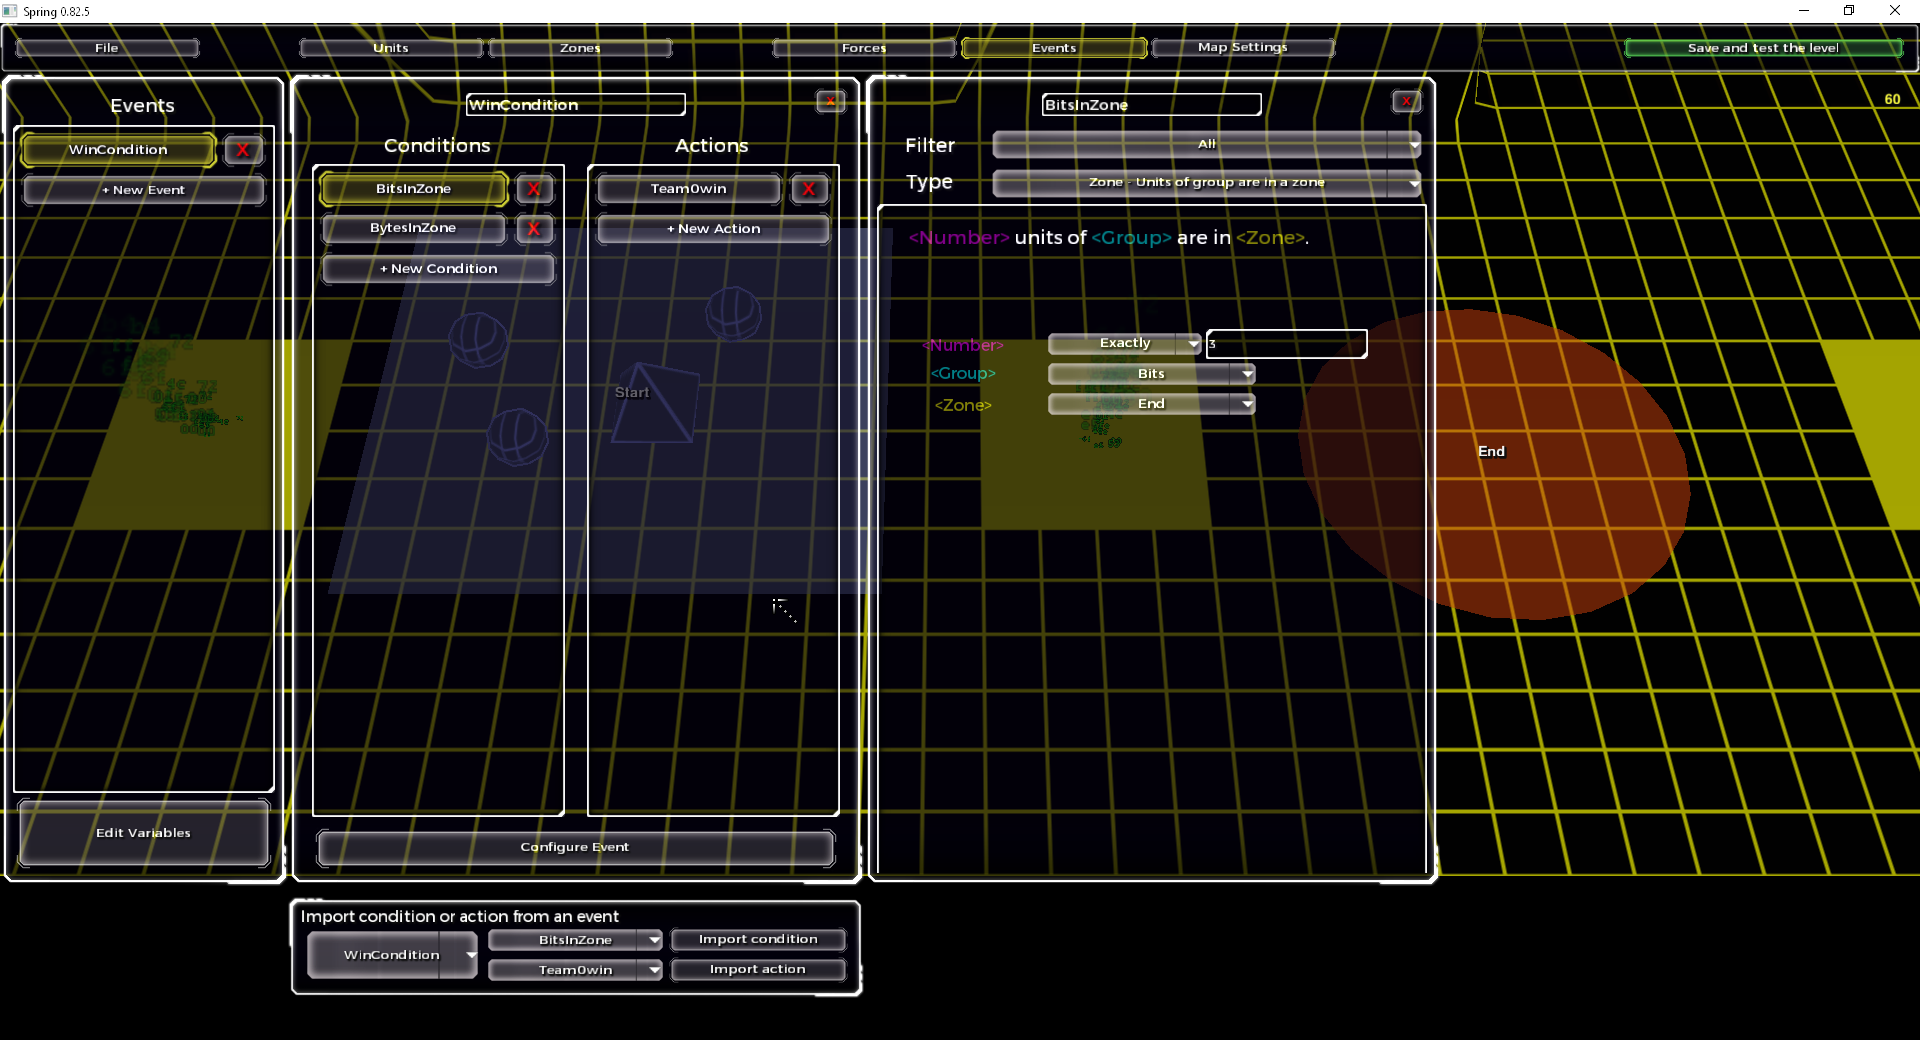
\includegraphics[width=\linewidth]{editor-trigger.png}
\caption{Exemple d'édition de la condition \textit{BitsInZone} de l'événement \textit{WinCondition}.}
\label{fig:editor-trigger}
\end{figure}
\begin{figure}[H]
\centering
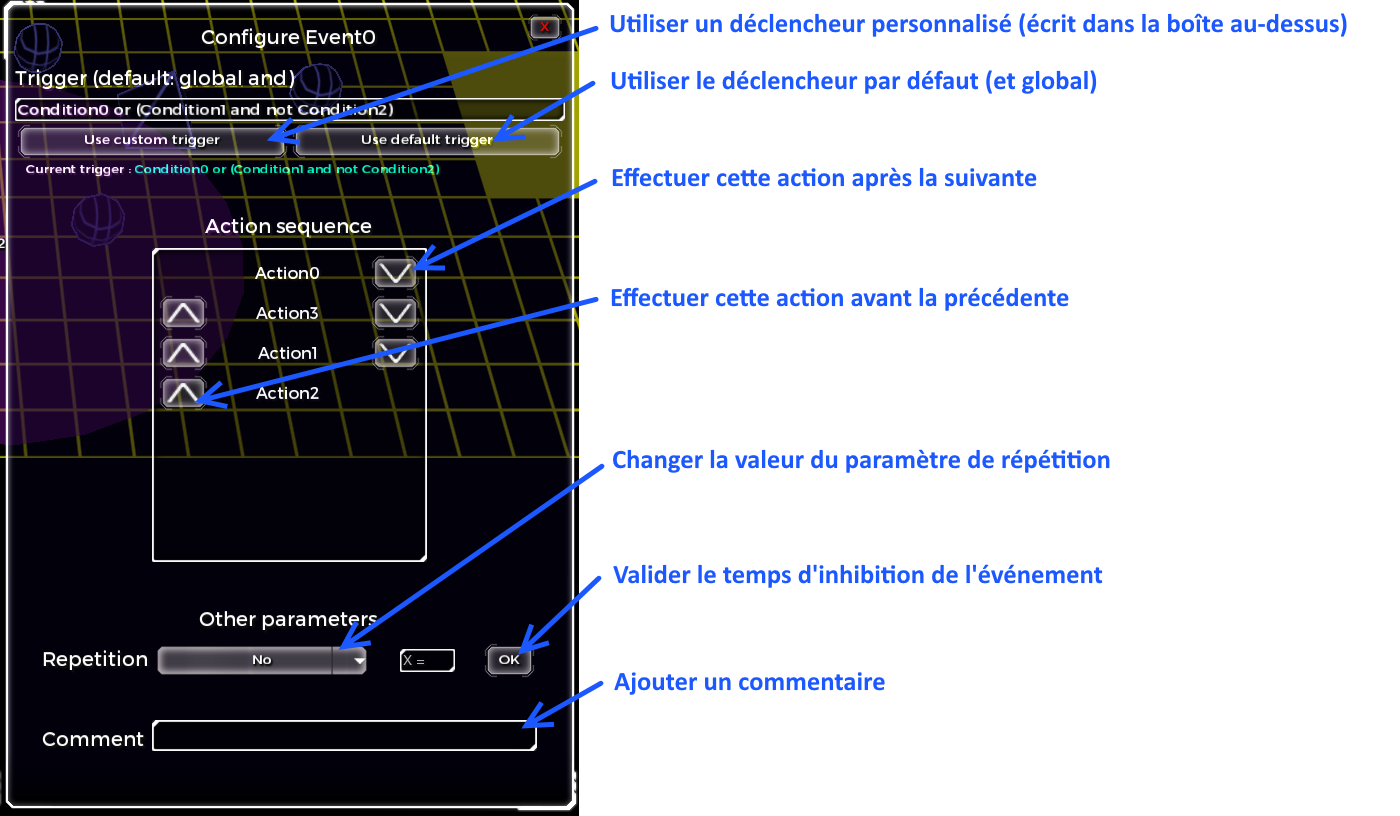
\includegraphics[width=\linewidth]{editor-eventconfig.png}
\caption{Interface de gestion d'un événement.}
\label{fig:editor-eventconfig}
\end{figure}
\subsubsection{Variables}
\paragraph{ }
L'éditeur d'évènements permet de définir des variables numériques ou booléennes. On accède à l'interface d'édition des variables en utilisant le bouton situé en dessous de la liste des évènements (Figure \ref{fig:editor-variables}). Ces variables permettent d'avoir plus de contrôle sur la façon dont s'enchaînent les différents évènements. Leurs valeurs peuvent être modifiées en utilisant des actions spécifiques aux variables.
\begin{figure}[H]
\centering
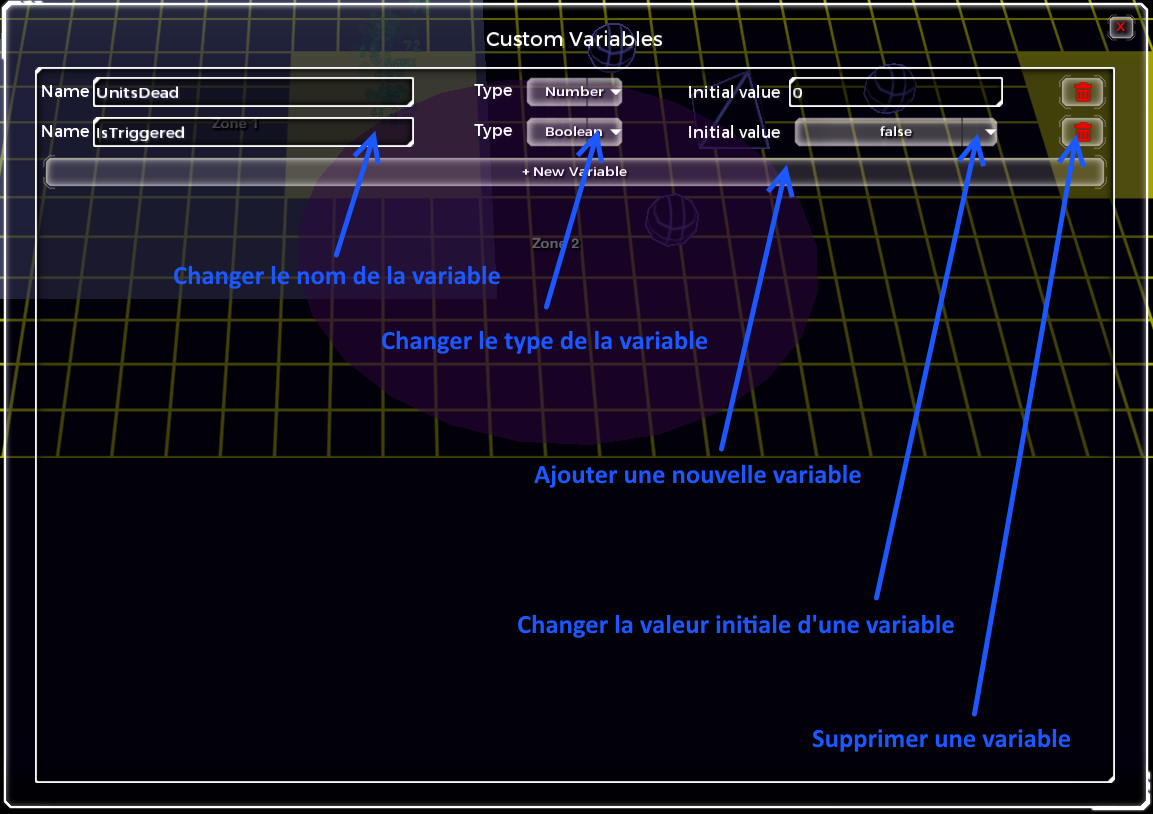
\includegraphics[width=\linewidth]{editor-variables.png}
\caption{Interface de gestion des variables.}
\label{fig:editor-variables}
\end{figure}
\subsubsection{Paramètres particuliers}
\paragraph{ }
Certains paramètres définissables dans les conditions et dans les actions requièrent des explications supplémentaires :
\begin{itemize}
\item \textbf{UnitSet} - Un ensemble d'unité correspond soit à une unité déjà présente dans la scène, soit à une équipe toute entière, soit à un groupe d'unités, soit aux unités validant une condition faisant parti de l'événement actuellement modifié, soit aux unités ayant été créées par le dernier appel à une action de création d'unité (voir Figure \ref{fig:editor-pickunit}). Une fois qu'une unité a été sélectionnée, il est possible de zoomer dessus en cliquant sur le bouton avec l'œil.
\item \textbf{Position} - Une position peut être soit un couple (x, y), soit une position aléatoire à l'intérieur d'une zone. Une fois qu'une position a été sélectionnée, il est possible de zoomer dessus en cliquant sur le bouton avec l'œil.
\item \textbf{Script} - Les paramètres de ce type s'adressent à des utilisateurs avancés. Le champ texte permet d'écrire du code en Lua permettant de définir totalement une condition\footnote{Le script défini dans le cas d'une condition doit nécessairement renvoyer une valeur booléenne.} ou une action personnalisée.
\end{itemize}
\begin{figure}[H]
\centering
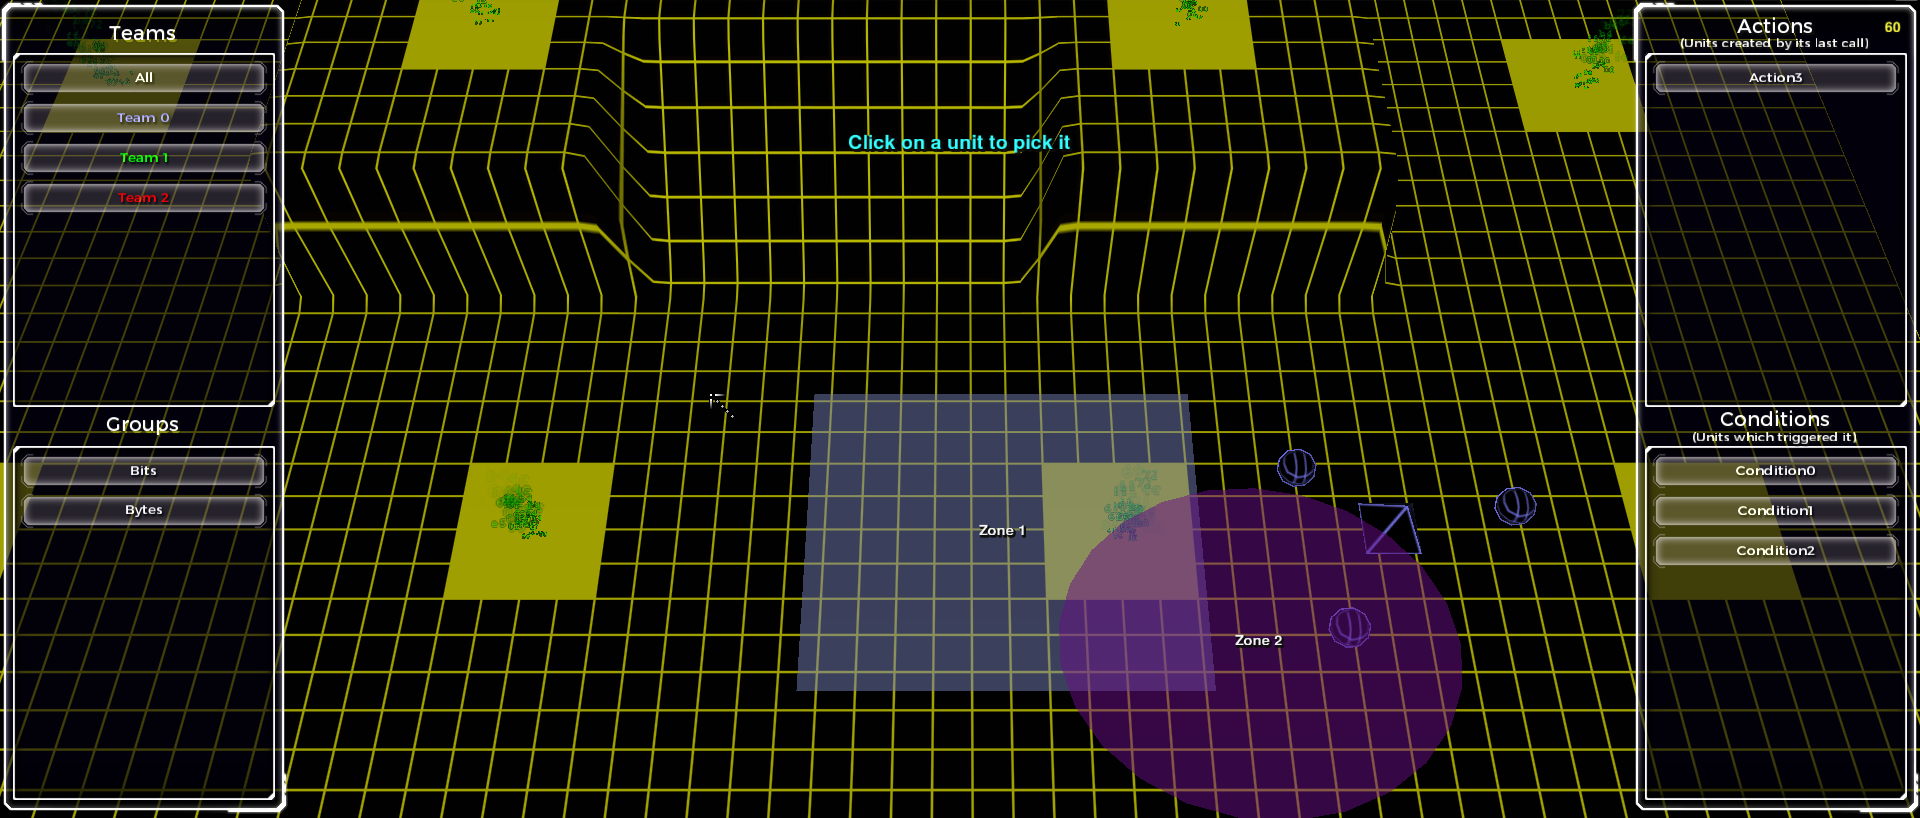
\includegraphics[width=\linewidth]{editor-pickunit.png}
\caption{Interface de sélection d'un UnitSet.}
\label{fig:editor-pickunit}
\end{figure}
\subsection{Paramètres de la carte}\label{mapsettings}
\paragraph{ }
Ce menu permet de choisir un nom pour le niveau, d'écrire un briefing qui sera affiché au début de la mission, et de spécifier certains paramètres (Figure \ref{fig:editor-mapsettings}).
\paragraph{ }
Le briefing peut contenir du texte coloré. Il faut pour cela choisir une couleur grâce aux sliders, sélectionner le texte à colorer, puis appuyer sur le bouton correspondant.
\paragraph{ }
Il est également possible d'activer ou de désactiver :
\begin{itemize}
\item la caméra automatique (en jeu, cette caméra contient en permanence dans son champ de vision les unités visibles par le joueur ainsi que les zones définies comme toujours présentes dans le champ de vision)
\item le soin automatique des unités
\item la souris
\item la minimap
\item certains widgets propres au mod sélectionné ou à Prog \& Play
\end{itemize}
\begin{figure}[H]
\centering
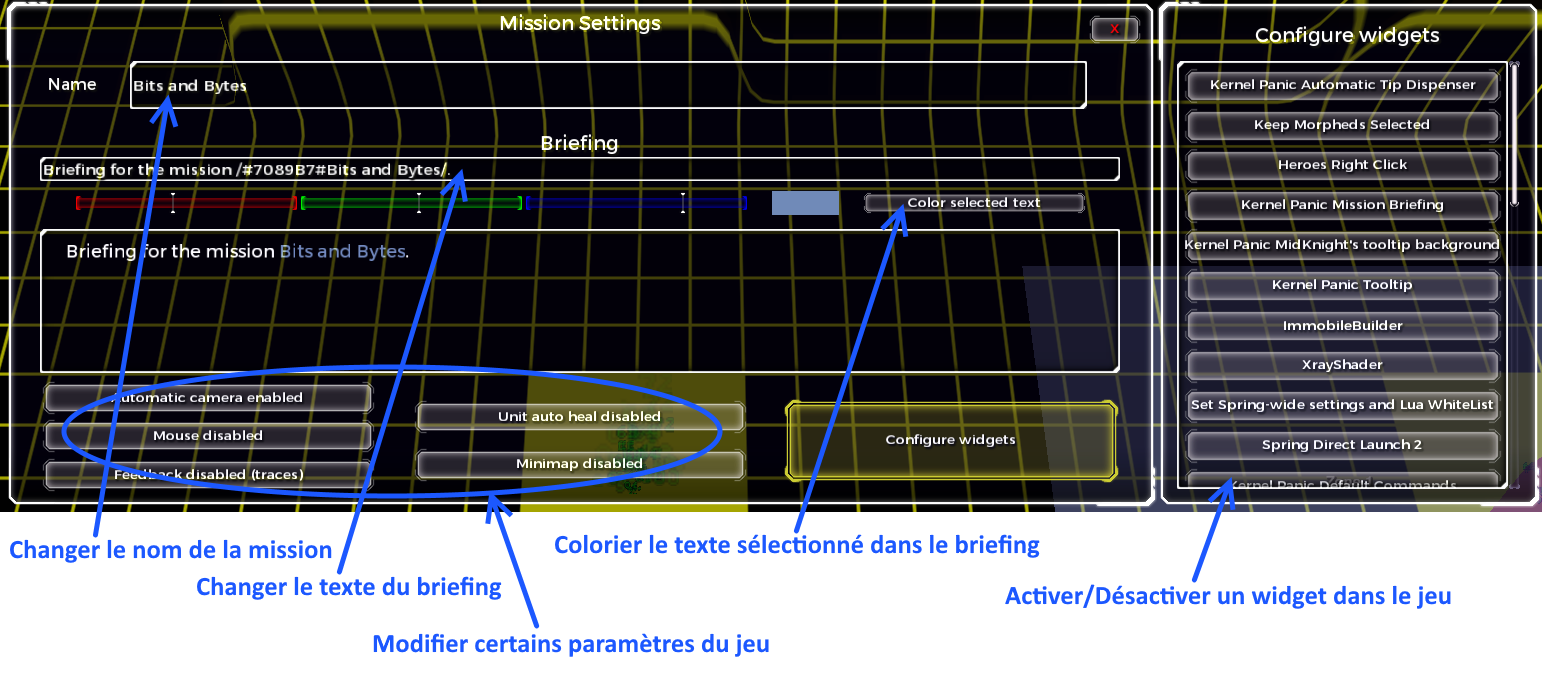
\includegraphics[width=\linewidth]{editor-mapsettings.png}
\caption{Interface de modification des paramètres de la mission.}
\label{fig:editor-mapsettings}
\end{figure}
\section{Création du jeu final}
\subsection{Scénario et exportation}\label{scenario-editor}
\paragraph{ }
Chaque niveau créé est représenté par une fenêtre contenant le nom du niveau, un état d'entrée et un ou plusieurs états de sortie en fonction de ce qui a été défini dans l'éditeur. En cliquant sur le bouton correspondant à un état de sortie puis sur le bouton correspondant à un état d'entrée, les deux états seront connectés. Vous pouvez double-cliquer sur un état de sortie pour supprimer le lien associé.
\paragraph{ }
Il est possible de sauvegarder et de charger des scénarios (ces derniers se trouvant dans le répertoire \textit{<Spring>/pp\_editor/scenarios}). 
\paragraph{ }
Enfin, la génération de l'archive finale du jeu créé avec les différentes missions et la scénarisation se fait en cliquant sur le bouton d'exportation du jeu\footnote{A noter qu'il est possible d'inclure tous les niveaux présents dans le répertoire \textit{/pp\_editor/missions/} même s'ils ne sont pas dans le scénario (niveaux bonus ou absence de scénarisation par exemple)}. L'archive se trouvera dans le répertoire \textit{<Spring>/mods} (82.5.1) ou \textit{<Spring>/games} (98+) Un exemple d'édition d'un scénario est disponible Figure \ref{fig:launcher-scenario}.
\begin{figure}[H]
\centering
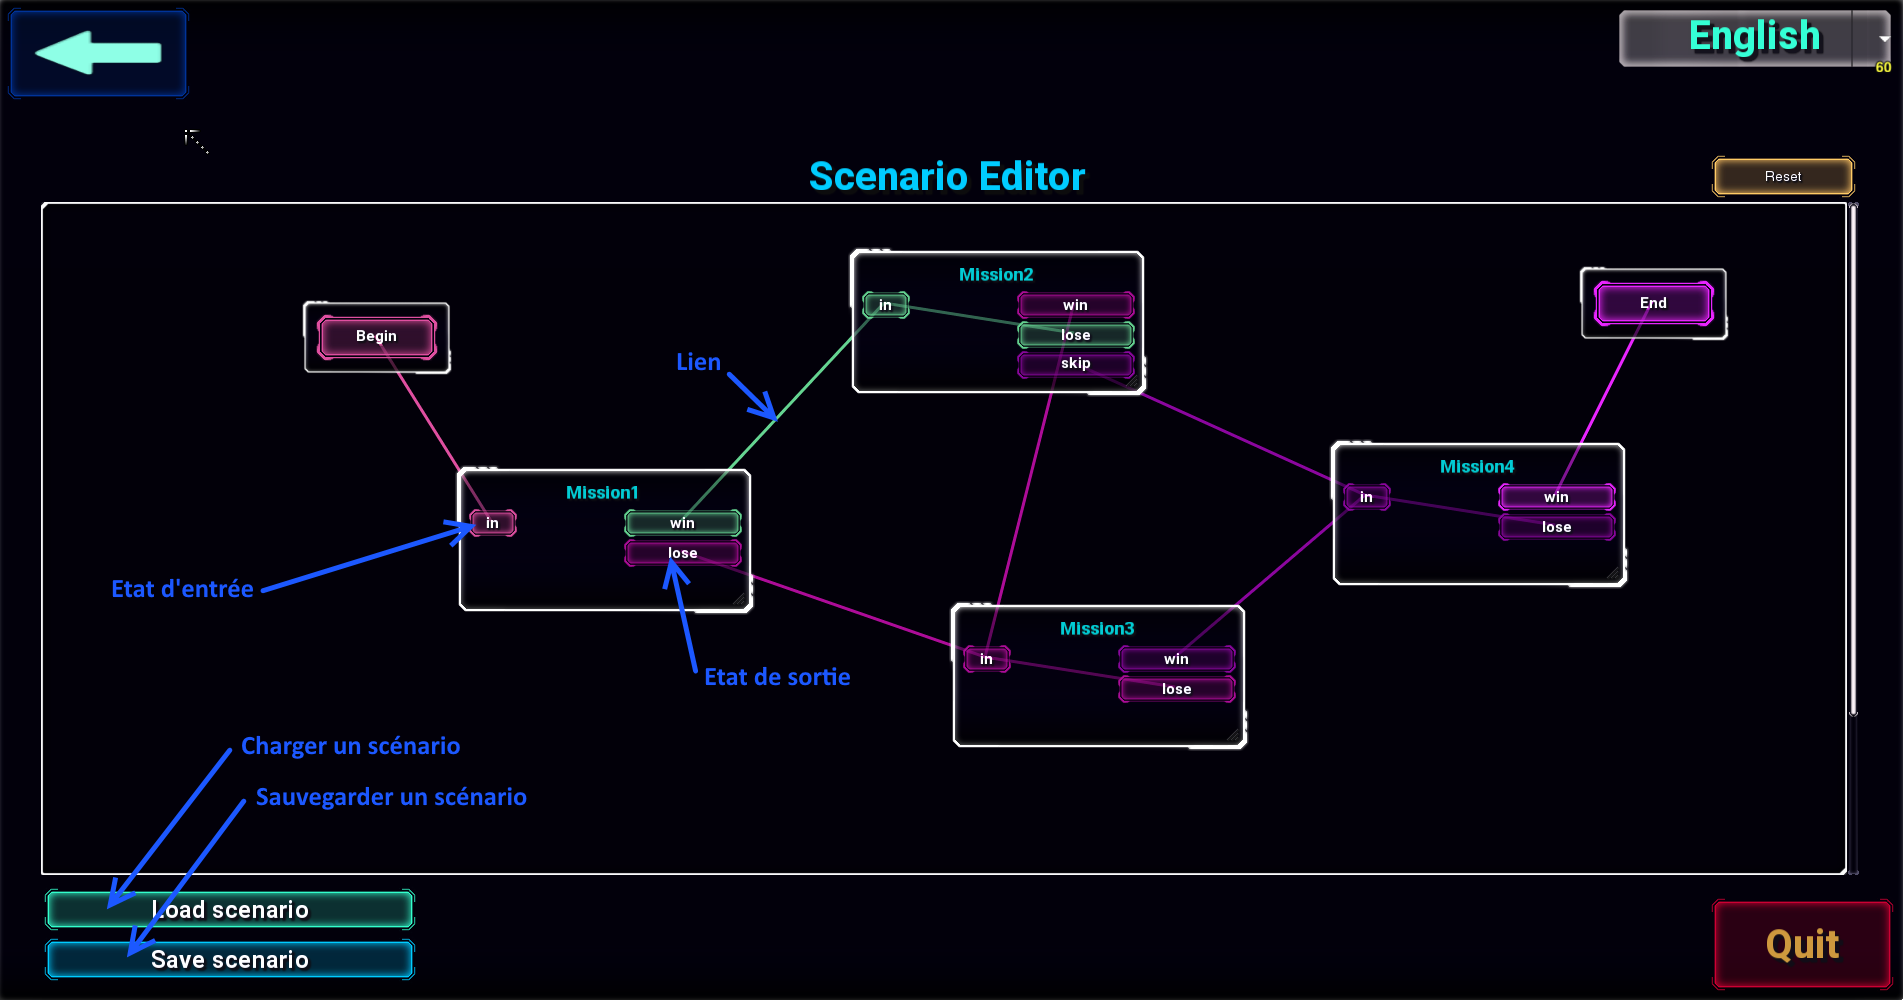
\includegraphics[width=\linewidth]{launcher-scenario.png}
\caption{Exemple d'édition d'un scénario à 3 missions.}
\label{fig:launcher-scenario}
\end{figure}
\subsection{Lancement du jeu créé}
\paragraph{ }
Une fois que les niveaux ont été créés, que le scénario a été défini et que le jeu a été packagé, il devient jouable. Il suffit alors de le placer dans le répertoire \textit{<Spring>/mods/} (82.5.1) ou \textit{<Spring>/games/} (98+) accompagné du jeu duquel il dépend (Kernel Panic 4.1 par exemple). Ensuite, il suffit de lancer Spring et de sélectionner le mod correspondant.
\paragraph{ }
Pour jouer en utilisant l'API Prog \& Play (et contrôler les unités par des lignes de code), assurez-vous de bien posséder une version de Spring intégrant Prog \& Play\footnote{Disponible sur \url{https://www.irit.fr/ProgAndPlay/}.}.
\end{document}
